\section{Projection mapping}\label{sec:projection-mapping}

Projection mapping is a spatial augmented reality \cite{Bimber2005} technique in which video projectors are used to overlay virtual geometry on top of real objects or surfaces. This allows to create an immersive environment that together with 3D perception systems can be used to develop interactive interfaces that show contextual information for helping or teaching human operators performing complex tasks faster. The next sections describe the mathematical projector modeling and the associated calibration that is necessary for performing proper 3D rendering of the virtual world in order to achieve high accuracy projection.


\subsection{Projector modeling}

The mathematical modeling of a \gls{dlp} projector can be seen as an inverse pinhole camera \cite{Hartley2003}, given the grid disposition of the mirrors in the \gls{dmd} and the very low distortion that modern \gls{dlp} projectors have. As such, scene rendering can be performed efficiently using the \gls{opengl} projection matrix (shown in \cref{eq:projection-matrix,eq:ndc-matrix,eq:perspective-matrix}), which incorporates the focal lengths (Fx, Fy), principal point (Cx, Cy) and axis skew (S) intrinsic camera parameters (in pixel units). The correction of lens distortion for \gls{dlp} projectors typically uses 3 coefficients for removing radial distortions and 2 coefficients for accounting for the tangential distortions.

{
	\scriptsize
	\begin{equation}\label{eq:projection-matrix}
	ProjectionMatrix = \glsentrytext{ndc}Matrix \times PerspectiveMatrix
	\end{equation}
	
	\begin{equation}\label{eq:ndc-matrix}
	NDCMatrix = 
	\begin{bmatrix}
	\frac{2}{ImageWidth} & 0 & 0 & -1 \\
	0 & \frac{2}{ImageHeight} & 0 & -1 \\
	0 & 0 & \frac{-2}{ClipFar - ClipNear} & \frac{-(ClipFar + ClipNear)}{ClipFar - ClipNear} \\
	0 & 0 & 0 & 1
	\end{bmatrix}
	\end{equation}
	
	
	\begin{equation}\label{eq:perspective-matrix}
	PerspectiveMatrix = 
	\begin{bmatrix}
	Fx & S & -Cx & 0 \\
	0 & Fy & -Cy & 0 \\
	0 & 0 & ClipNear + ClipFar & ClipNear \times ClipFar \\
	0 & 0 & -1 & 0
	\end{bmatrix}
	\end{equation}
}


\subsection{Projector calibration}

High accuracy projection mapping requires proper hardware / software calibration of the camera / projector and also appropriate positioning within the intended workspace in order to avoid occlusions caused by the objects 3D shape or the human operators. This calibration aims to compute the intrinsic parameters of the projector (that do not change when the projector is moved within the workspace) along with the extrinsic parameters that are needed to know where is the projector in the global reference frame in order to be able to do proper 3D rendering of the scene that will be projected.

The intrinsic parameters of a \gls{dlp} projector can be computed using image analysis of complementary gray code patterns projected into a chessboard. The calibration system proposed in \cite{Moreno2012} was used to retrieve the 5 intrinsic parameters (Fx, Fy, Cx, Cy, S) of the projector along with the 3D position and rotation of the projector in relation to the camera (that remains firmly attached to the projector support for fast recalibration of the extrinsic parameters). It was used 5 sets of 42 gray code image patterns captured with the chessboard in different positions and orientations in relation to the projector, that was pointing to the table workspace at a distance of 0.81 meters.

After having the intrinsic parameters of the camera and projector along with the relative position of the projector in relation to the camera, computing the global position of the projector in relation to the chessboard reference frame can be done by multiplying the $4 \times 4$ homogeneous matrix that gives the transformation from the chessboard origin to the camera frame, with the $4 \times 4$ homogeneous matrix that gives the transformation from the camera frame to the projector frame.



\subsection{Scene rendering}

For achieving accurate projection mapping, the Gazebo simulator\footnote{\url{http://gazebosim.org}} camera implementation was improved to allow the setting of a custom projection matrix in order to perform 3D rendering with a camera model that takes into account the projector intrinsic parameters. Moreover, it was added the possibility to dynamically change image, video and text during runtime for allowing the display of the relevant information for each assembly step.

For efficient 3D scene rendering, the Gazebo simulator relies on the cross platform open source Ogre3D graphics engine\footnote{\url{http://www.ogre3d.org}}, that in turn uses the \gls{opengl} \gls{gpu} \gls{api} to take advantage of the massively parallel graphics cards currently available to generate raster images for the \gls{dlp} projector.

For user interface, the Gazebo simulator has a Qt\footnote{\url{https://www.qt.io/}} \gls{gui} that allows visual inspection of the scene while also giving the option to add new objects or move and rotate existing models. Moreover, for lightweight rendering, it can also start in server mode without a \gls{gui}.



\section{Human machine interaction}\label{sec:human-machine-interaction}

The immersive \gls{hmi} system developed projects into the workspace detailed textual information of the current assembly task along with a video showing the operation being performed by an expert operator. Given the high variability of assembly / maintenance operations, the system was designed to decompose the assembly process into a set of small and concise operations. This allows to keep the operator focused on the current task and reduces the required projection area. Moreover, the operator can pause and move the video forwards and backwards, allowing to inspect a given complex operation with more time.

The user interaction with the projected \gls{hmi} is done by analyzing the 3D point cloud sensor data that falls within a set of \glspl{roi} (shown in \cref{fig:interaction-rois}). When a minimum number of points falls within a given \gls{roi}, the cluster of points centroid is extracted (shown as spheres in \cref{fig:interaction-rois}) and if this \gls{roi} is associated with a button, the user needs to hold the finger for at least 0.25 seconds to trigger the action. Moreover, to avoid unintentional action triggering, the user needs to remove and insert the finger into the \gls{roi} to request the action again. On the other hand, if the \gls{roi} is associated with the video seek bar \gls{roi} (the vertical yellow box in \cref{fig:interaction-rois}), the video seek time is computed considering the relative position of the finger within the \gls{roi} (the bottom of the \gls{roi} is associated with the start of the current video while the top corresponds to the end of the current video).

Besides video play / pause functionality (provided by the blue middle \gls{roi} shown in \cref{fig:interaction-rois}), the \gls{hmi} also allows the operator to navigate within the assembly operations (using the green \glspl{roi} visible in \cref{fig:interaction-rois}). As can be seen in \cref{fig:human-machine-interface,fig:interaction-rois}, there are buttons for moving to the first, previous, next and last assembly step. Moreover, it is also shown what is the number of the current assembly step and how many steps are required to complete the assembly.

\begin{figure}[H]
	\begin{floatrow}[2]
		\ffigbox[1.4\FBwidth]
		{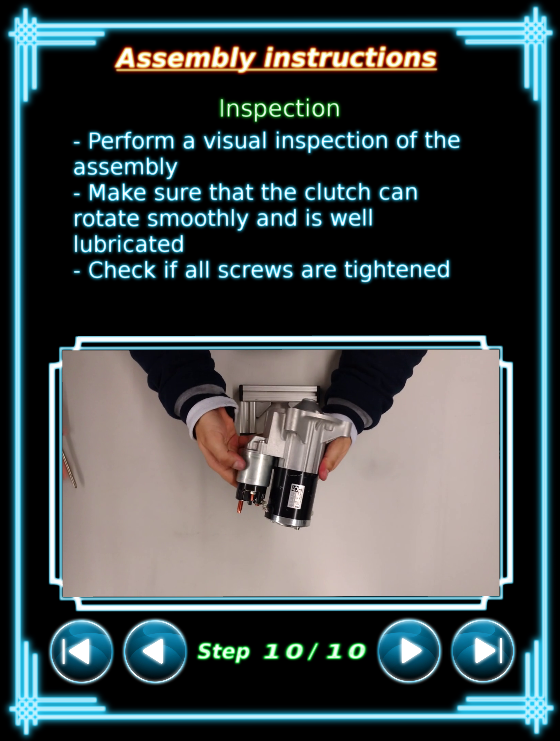
\includegraphics[height=.23\textheight]{human-machine-interface}}
		{\caption{Rendering of the human machine interface}\label{fig:human-machine-interface}}
		\ffigbox[1.8\FBwidth]
		{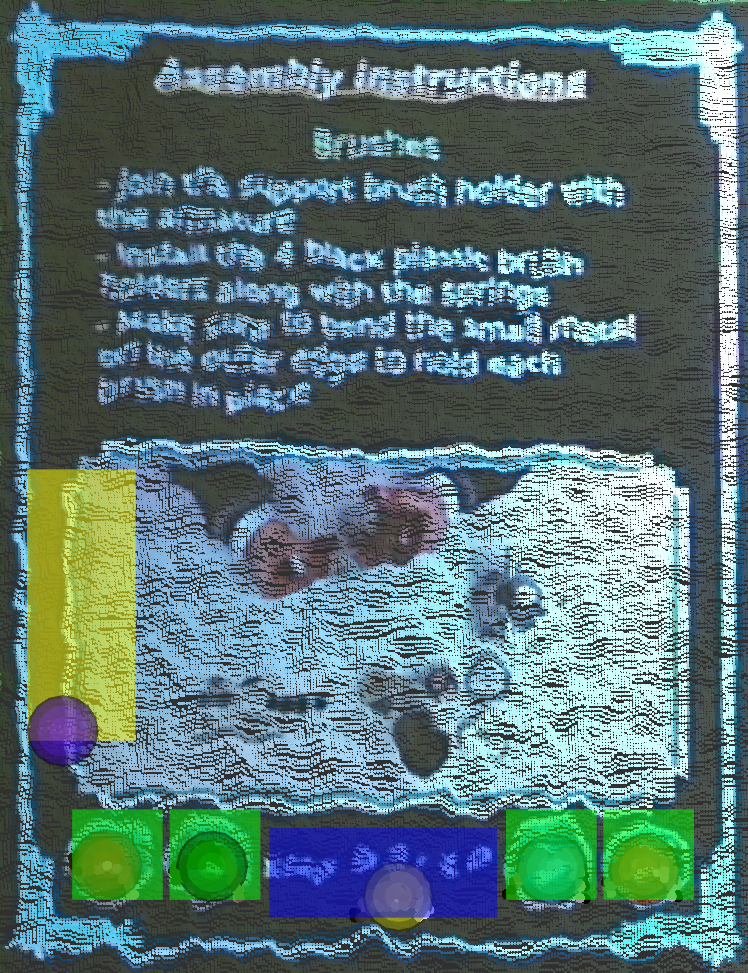
\includegraphics[height=.23\textheight]{interaction-rois}}
		{\caption{\glspl{roi} for the \gls{hmi} (overlaid on top of the Kinect 2 point cloud sensor data)}\label{fig:interaction-rois}}
	\end{floatrow}
\end{figure}



\section{Object recognition}\label{sec:object-recognition}

Robust and accurate object recognition and pose estimation is a requirement when developing projection mapping systems with dynamic objects. To achieve this goal, the 3D perception pipeline described in \cite{Costa2016} was fine tuned for our table top recognition use case. In \cref{fig:initial-pose-estimation} is shown the estimation of the pose of the starter motor. When the system started (left image), it subsampled the reference pointcloud (small green circles) and computed the \gls{sift} \cite{Lowe2004} keypoints (large yellow circles) and associated \gls{fpfh} \cite{Rusu2009} feature descriptors. Then, when sensor data arrived, it retrieved the points within a \gls{roi} above the workspace table, detected the keypoints (blue circles) and their descriptors and applied the feature matching and registration refinement, achieving the pose estimation showed on the right image of \cref{fig:initial-pose-estimation} (observe the overlap between the sensor data and the reference point cloud). After the successful initial pose estimation phase, the recognition system enters in tracking mode and relies only on point cloud matching algorithms (given their better accuracy and lower computational cost). If the tracking is lost, the feature matching algorithms are used again to find a plausible estimation of the object position that is then refined with the point cloud registration refinement algorithms.

\begin{figure}[!ht]
	\centering
	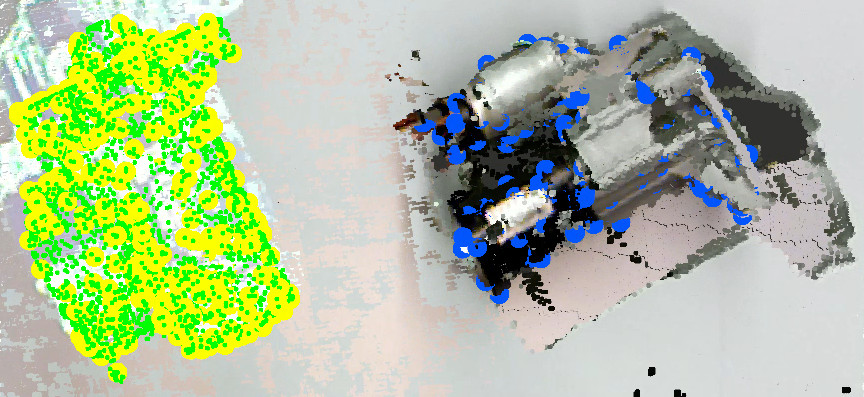
\includegraphics[height=.155\textheight]{initial-pose-estimation-2-before}
	\hspace{0.5em}
	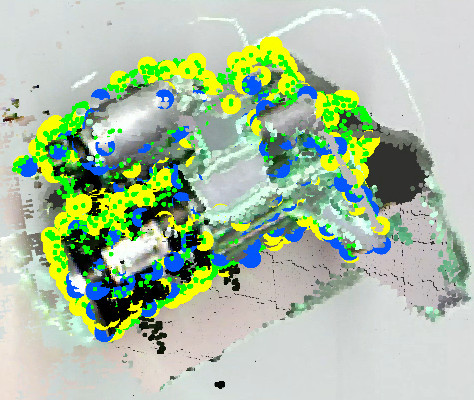
\includegraphics[height=.155\textheight]{initial-pose-estimation-2-after}
	\caption{Initial pose estimation of assembled starter motor}
	\label{fig:initial-pose-estimation}
\end{figure}
